\documentclass[tikz]{standalone}
\usepackage{tikz}
\usepackage{amsmath}
\usepackage{amsfonts}
\usetikzlibrary{arrows.meta, calc}

% The cover. Compiles on its own to cover.pdf, which \cover{cover.pdf} picks up.
%
% Two constraints worth knowing before you draw:
%
%   1. The frame below sets the page size. It is 10.4 by 7.2, a ratio of 1.44. The title
%      page scales the image to the full text width, so a much taller or wider drawing
%      will not fit alongside the title. Keep the ratio near 1.45.
%
%   2. Keep it to two colours. One for the thing the tutorial is about, one for whatever
%      it is contrasted with. The finished covers use red!60!orange and blue!50!cyan.
%
% Anchors of an empty 16x11 page are fine to leave in; what matters is the frame.

\begin{document}
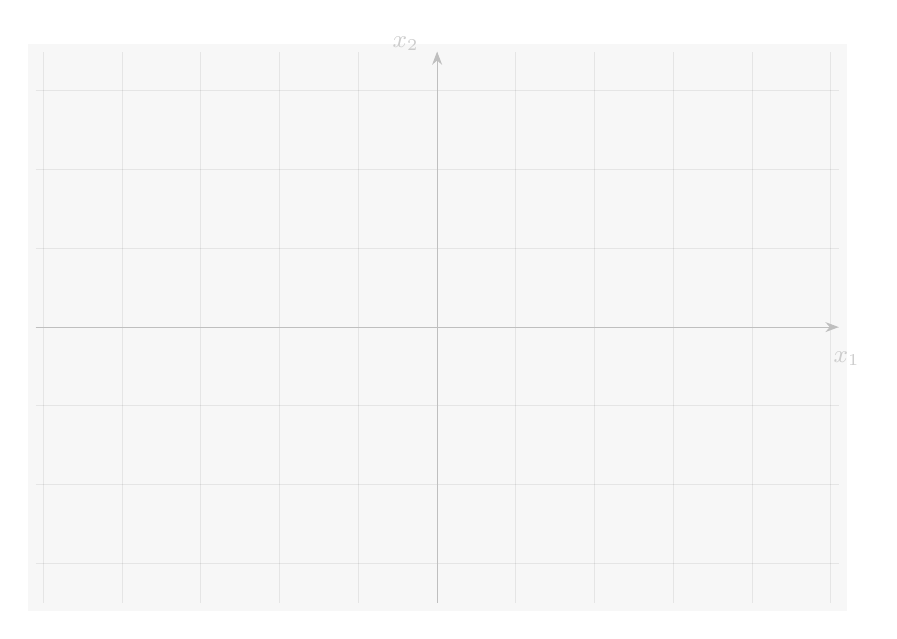
\begin{tikzpicture}[>=Stealth]

  % ---- canvas ----
  \fill[gray!6] (-5.2,-3.6) rectangle (5.2,3.6);

  % A barely visible reference grid.
  \begin{scope}[opacity=0.07]
    \foreach \x in {-5,...,5} { \draw[black, thin] (\x,-3.5) -- (\x,3.5); }
    \foreach \y in {-3,...,3} { \draw[black, thin] (-5.1,\y) -- (5.1,\y); }
  \end{scope}

  % Axes.
  \draw[->, black!25, thin] (-5.1,0) -- (5.1,0);
  \draw[->, black!25, thin] (0,-3.5) -- (0,3.5);
  \node[black!20, font=\small] at (5.2,-0.4) {$x_1$};
  \node[black!20, font=\small] at (-0.4,3.6) {$x_2$};

  % ---- your drawing goes here ----
  % What the three finished covers do, for reference:
  %
  %   Convex Optimization  contour ellipses of a convex function, with a zigzagging
  %                        gradient-descent path and a stepped FISTA path converging
  %   Compressed Sensing   the measurement equation Y = Phi Psi^T X drawn as a diagram
  %   Linear Algebra       a unit grid sheared by a matrix, with the standard basis and
  %                        the columns of that matrix drawn on top

\end{tikzpicture}
\end{document}
